\section*{Problema 2}
\textbf{Cuál es la probabilidad de que el segmento seleccionado en la figura \ref{fig:circle_problem2} tenga una longitud mayor que $\sqrt{3}$?}
\begin{figure}[H]
    \centering
    \begin{minipage}{5cm}
        \centering
        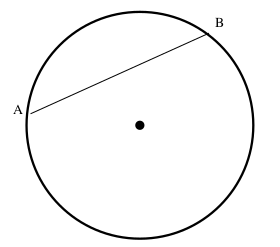
\includegraphics[width=4cm,height=3.5cm]{Graphics/circle_problem2.png}
        \caption{}
        \label{fig:circle_problem2}
    \end{minipage}
    \begin{minipage}{5cm}
        \centering
        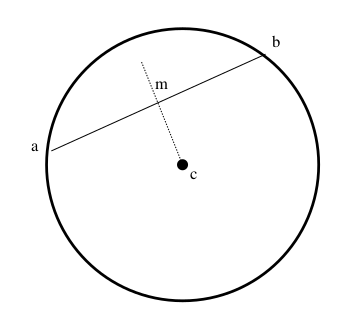
\includegraphics[width=4cm,height=3.5cm]{Graphics/circle_2a.png}
        \caption{}
        \label{fig:circle_m}
    \end{minipage}
    \begin{minipage}{5cm}
        \centering
        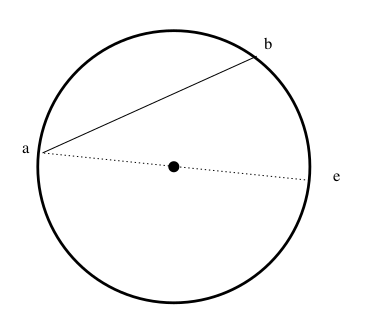
\includegraphics[width=4cm,height=3.5cm]{Graphics/circle_2b.png}
        \caption{}
        \label{fig:circle_angle}
    \end{minipage}
\end{figure}
\begin{itemize}
    \item \textbf{Una primera interpretación está basada en el hecho de que cualquier segmento está caracterizado de una manera única por el punto en la intersección del segmento con la recta ortogonal al segmento y que pasa por el centro (ver el punto m en figura \ref{fig:circle_m}). Así podemos construir un segmento eligiendo ese punto m al azar dentro del círculo. Calcula bajoesta interpretación la probabilidad de tener un segmento mayor que $\sqrt{3}$.}

          En esta interpretación cada linea trazada sobre el circulo sera rotada hasta que esta sea perpendicular a la linea m. Al nosotros querer lineas mayores a $\sqrt{3}$, calcularemos el valor de m correspondiente a esta medida a la cual llamaremos $m_{max}$.
          \begin{align*}
              m_{max} & = \sqrt{1-\left(\frac{3}{2}\right)} \\
                      & = \sqrt{1-\frac{3}{4}}              \\
                      & = \sqrt{\frac{1}{4}}                \\
              m_{max} & = \frac{1}{2}
          \end{align*}
          entonces, se tiene que para $m<\frac{1}{2}$ se obtienen longitudes mayores a $\sqrt{3}$. En la figura \ref{fig:problema2_interpretacion1}, las lineas verdes tienen un $m<m_{max}$ y las rojas son $m>m_{max}$.
          \begin{figure}[H]
              \centering
              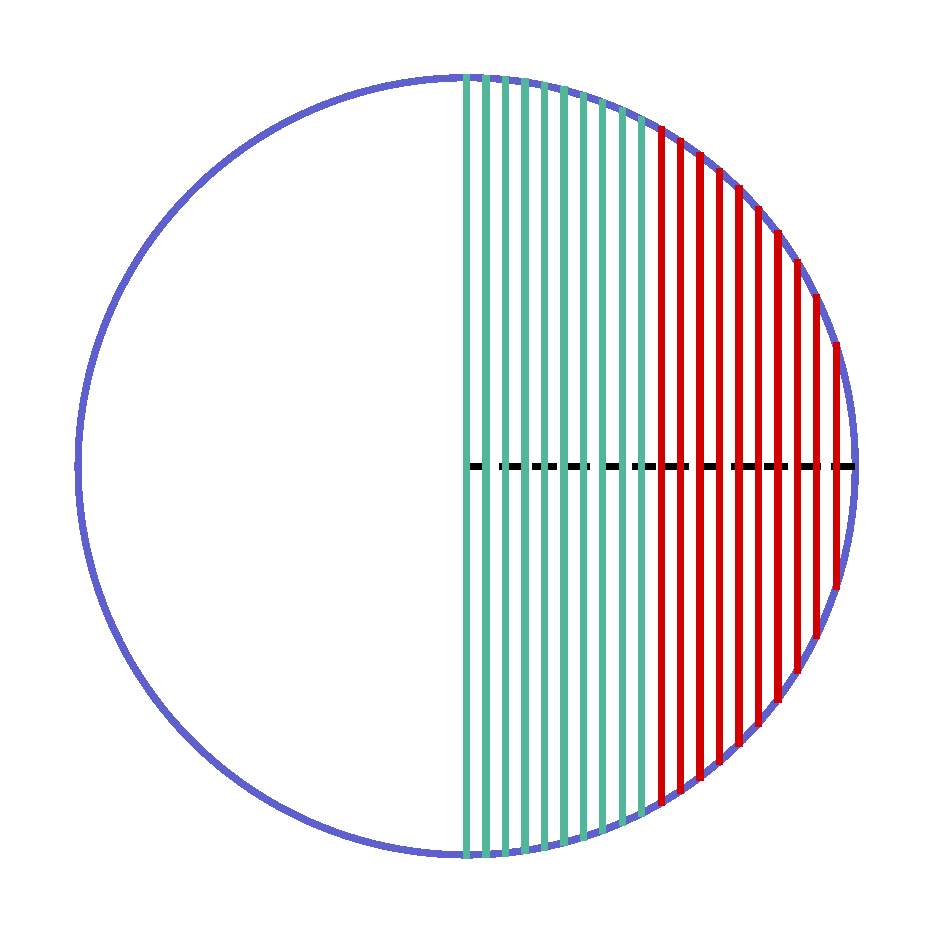
\includegraphics[width=6cm]{Graphics/circle_2.eps}
              \caption{}
              \label{fig:problema2_interpretacion1}
          \end{figure}
          Como el radio del circulo es 1, entonces, la probabilidad de obtener una linea con longitud mayor es:
          \begin{align*}
              P(d>\sqrt{3}) & = \frac{\dfrac{1}{2}}{1} \\
              P(d>\sqrt{3}) & = \frac{1}{2}
          \end{align*}
          Por lo tanto, la probabilidad de obtener una linea con una longitud mayor a $\sqrt{3}$ es $\frac{1}{2}$.
\end{itemize}
\begin{itemize}
    \item \textbf{En otra interpretación, fijamos primero el punto a en el círculo y elegimos al azar otro punto (b) en el círculo y definimos el segmento como la linea entre a y b (ver figura \ref{fig:circle_angle}). Para que el segmento tenga una longitud mayor que $\sqrt{3}$: ¿ qué restricción hay para el ángulo abe ?. En base a eso, calcula la probabilidad de tener un segmento mayor que $\sqrt{3}$.}

          Observando la figura \ref{fig:circle_angle}, se forma un triangulo rectangulo con los puntos a,b y e. La distancia del punto al e es d, que en este caso es 2. Al querer una distancia mayor a $\sqrt{3}$ entre los puntos ab. Calcularemos el angulo abe conn estas distancias.
          \begin{align*}
              Cos(\theta) & = \frac{\sqrt{3}}{2} \\
                          & = 0.86602            \\
              \theta      & = 30
          \end{align*}
          Como queremos distancias mayores a $\sqrt{3}$, entonces esto sucedera para ángulols menores a $30$. Como la función coseno es par, entonces nuestro rango de valores admitidos estan en el rango $\theta' \in[-30,30]$. Como el rango de valores que podemos tener en la figura \ref{fig:circle_angle} es [-90,90], entonces la probabilidad con esta interpretación es
          \begin{align*}
              P(-30<\theta<30) & = \frac{60}{180} \\
                               & = \frac{1}{3}
          \end{align*}
          En la figura \ref{fig:problema2_interpretacion2} se representan algunas lineas con esta interpretación. Las lineas verdes y rojas representan aquellas que tienen una distancia mayor o menor a $\sqrt{3}$ respectivamente.
          \begin{figure}[H]
              \centering
              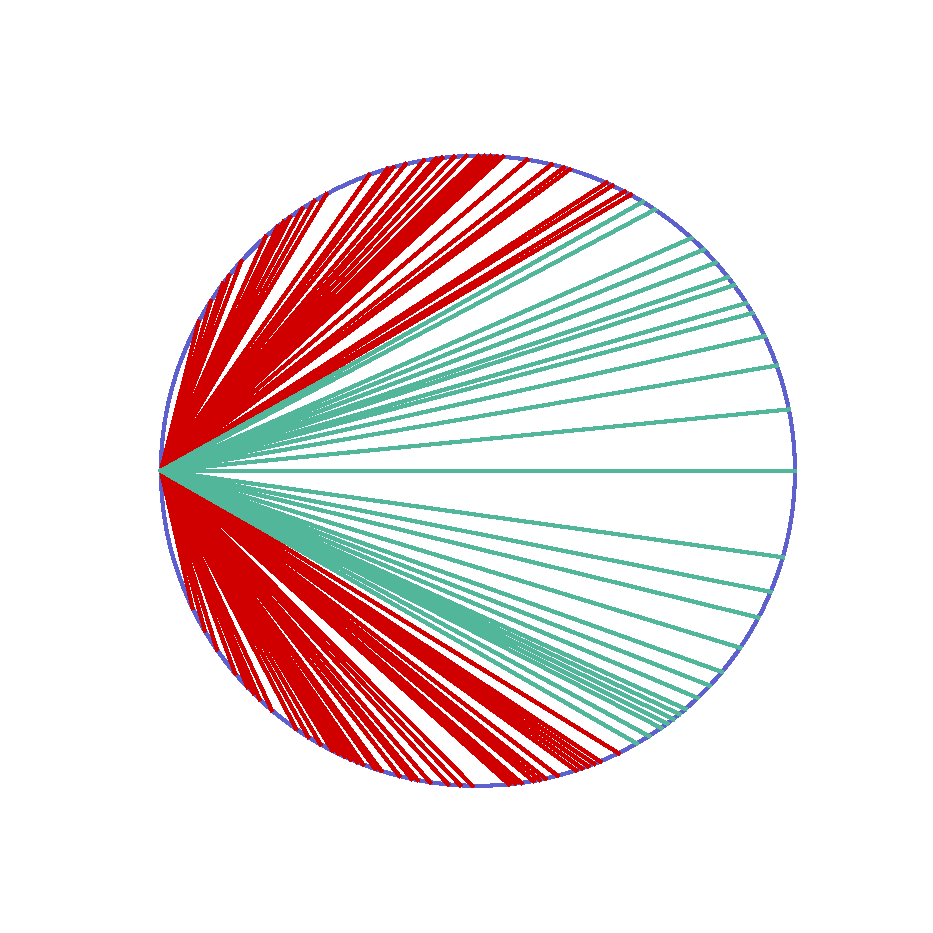
\includegraphics[width=6cm]{Graphics/circle_4.eps}
              \caption{}
              \label{fig:problema2_interpretacion2}
          \end{figure}
\end{itemize}
\begin{figure}[H]
    \centering
    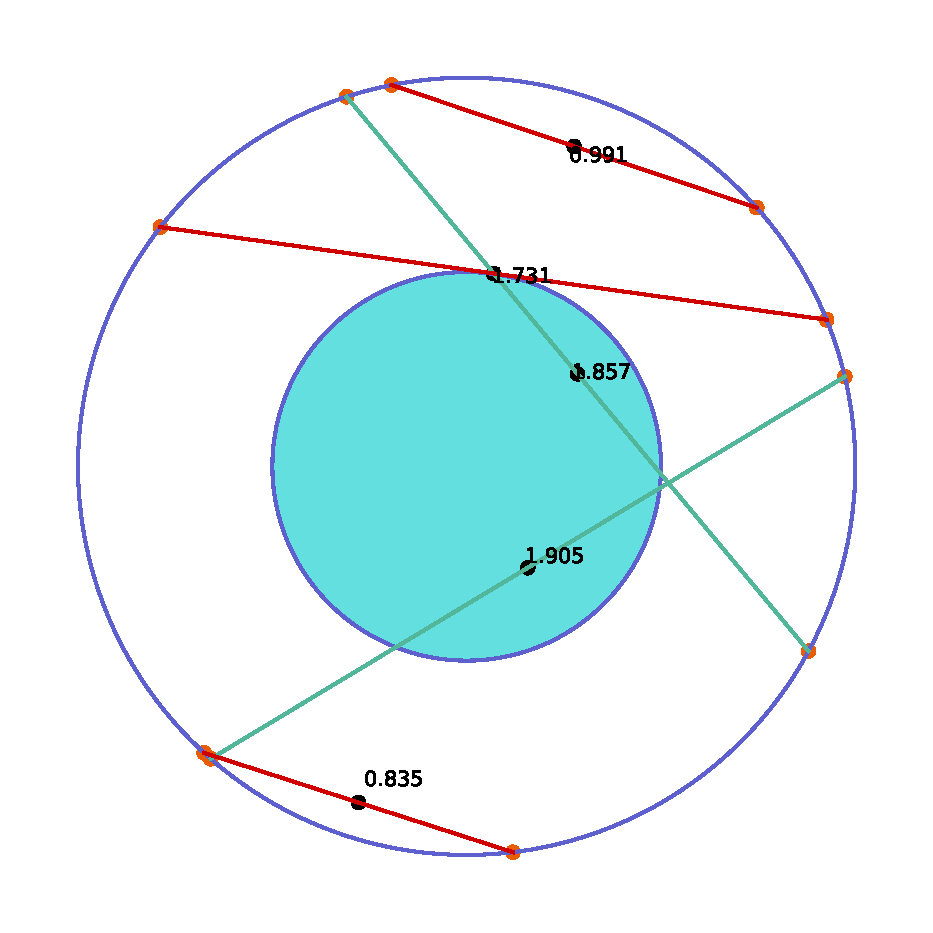
\includegraphics[width=7cm]{Graphics/circle_3_1.eps}
    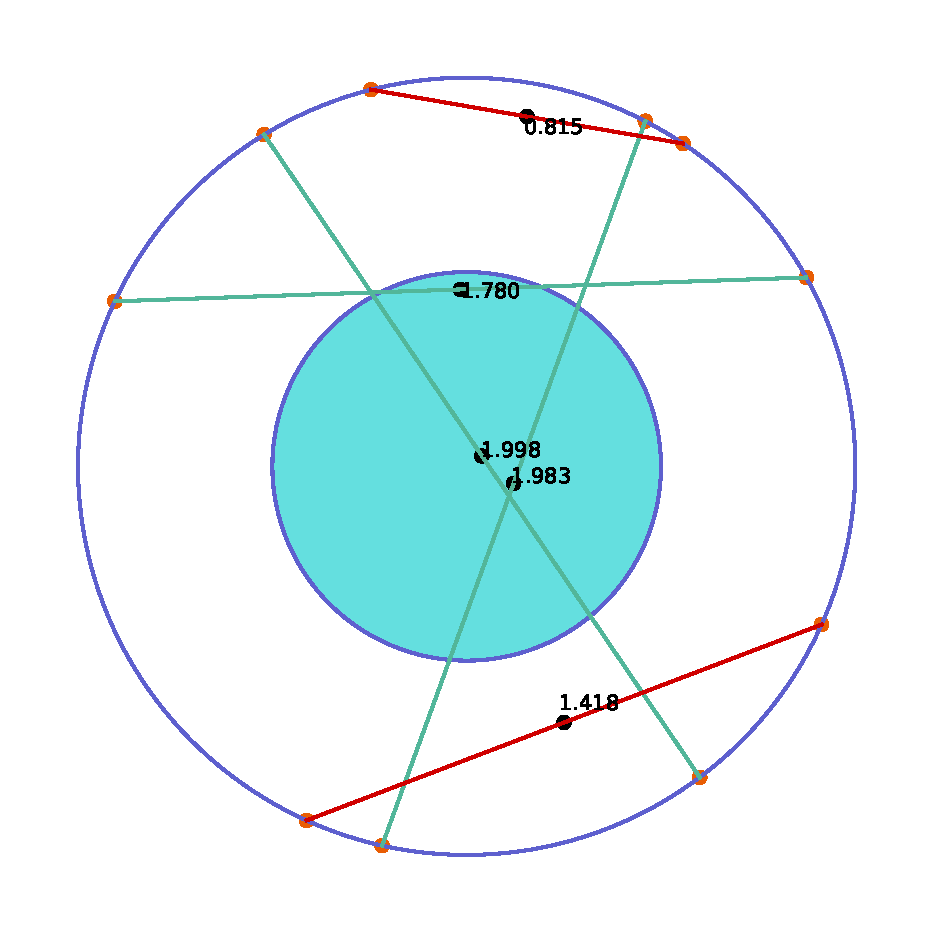
\includegraphics[width=7cm]{Graphics/circle_3_2.eps}
    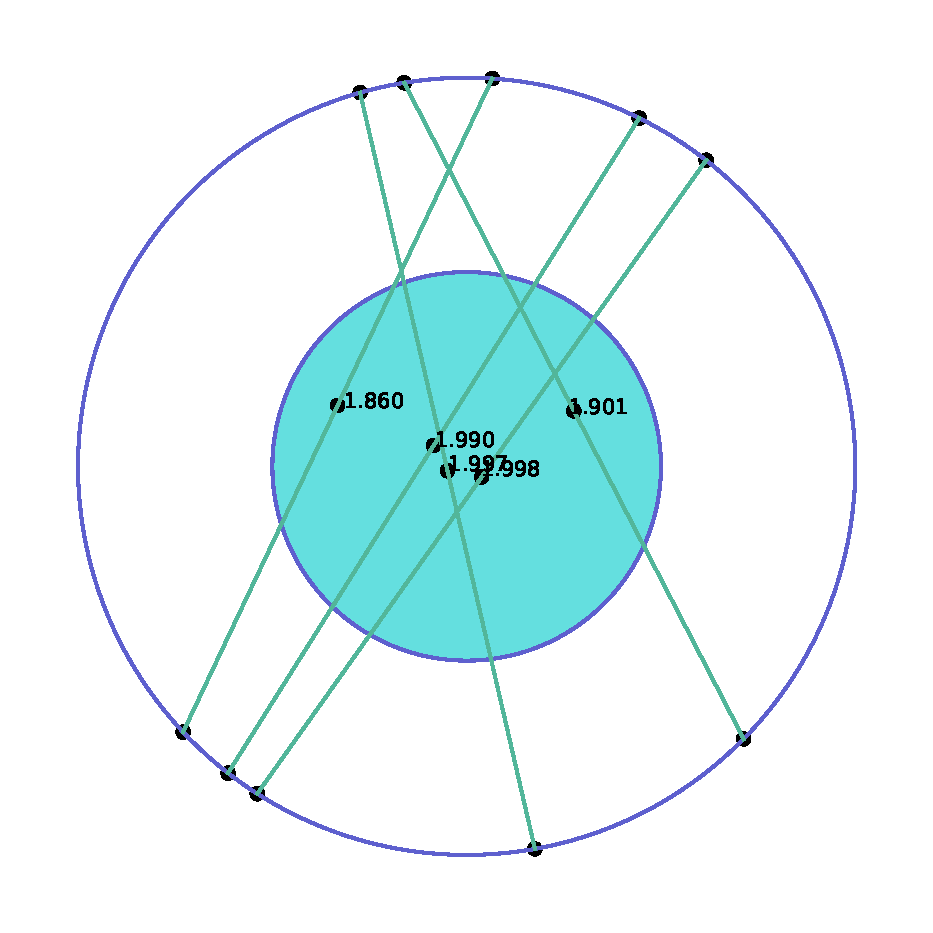
\includegraphics[width=7cm]{Graphics/circle_3_3.eps}
    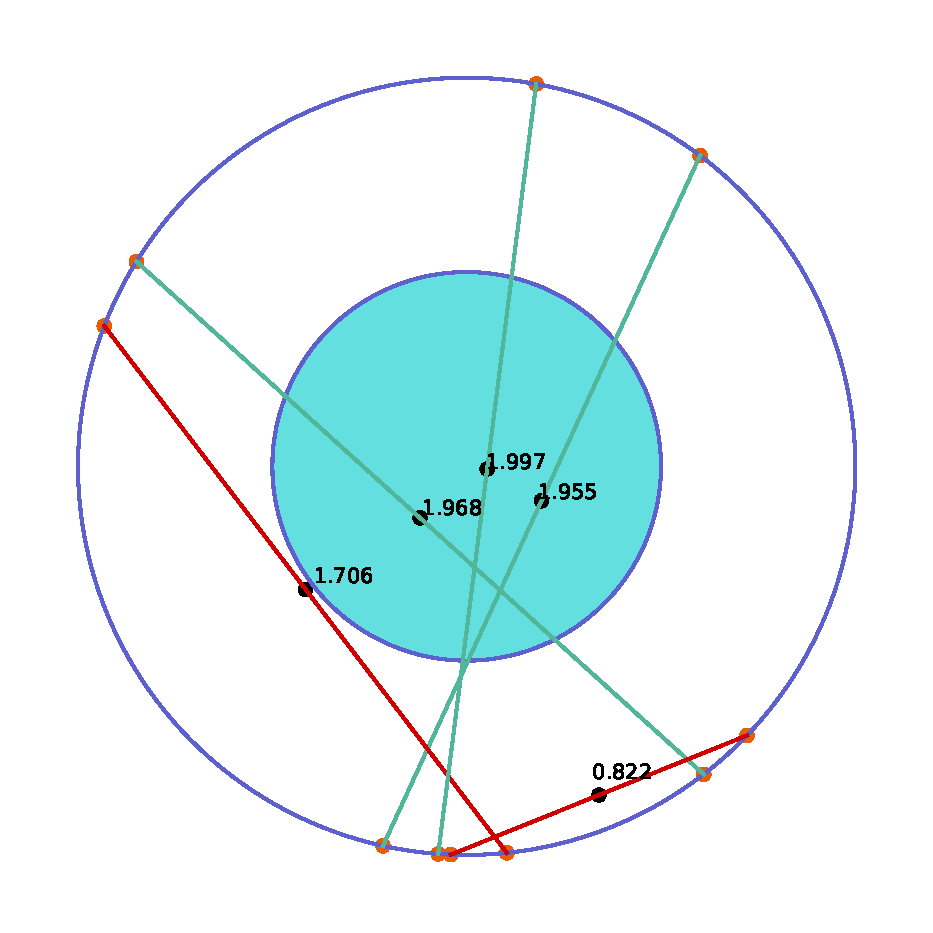
\includegraphics[width=7cm]{Graphics/circle_3_4.eps}
    \caption{}
\end{figure}